\subsection{Theorem von Gell-Mann und Low}
\subsubsection*{Berechnung von Erwartungswerten im Grundzustand}
\begin{equation}
  \begin{aligned}
    \erw{A(t)} & = \bra{\phi_G}A_H(t)\ket{\phi_G}                   \\
               & = \bra{\phi_G}S(t_0,t) A_0(t) S(t,t_0)\ket{\phi_G}
  \end{aligned}
\end{equation}

Hierbei beschreibt $S(t,t_0)$ die Zeitentwicklung des Systems unter Einfluss von $H_{\mathrm{int}}$ im
Wechselwirkungsbild, also die Entwicklung von $t_0$ nach $t$. Der Operator $S(t_0,t)$ beschreibt die Zeitentwicklung
von $t$ zurück nach $t_0$.

Die Zeitentwicklung laesst sich als geschlossene Zeitkontur auffassen: oben laeuft die Entwicklung von $t_0$ nach $t$,
unten wieder zurueck von $t$ nach $t_0$.

\begin{figure}[htbp]
  \centering
  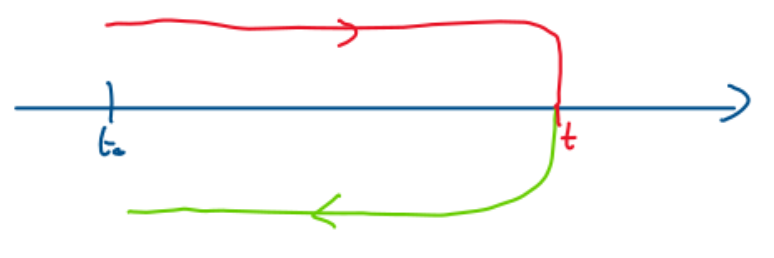
\includegraphics[width=0.82\linewidth]{Pictures/Gell-Mann_Timeordering_Problem.png}
  \caption{Skizze der Zeitentwicklung entlang der Kontur: der obere Ast ist zeitgeordnet und beschreibt die Entwicklung von $t_0$ nach $t$, der linke Ast ist antizeitgeordnet und fuehrt von $t$ wieder nach $t_0$.}
  \label{fig:gell-mann-low-kontur}
\end{figure}

Die Anwendung quantenfeldtheoretischer Methoden setzt dabei eine einheitliche Zeitordnung voraus.

$\rightarrow$ Ziel vom Theorem: die antizeitgeordneten Operatoren in zeitgeordnete Operatoren umzuwandeln.

\subsubsection*{zeitgeordnete GF in der WW-Darstellung}

\begin{equation}
  \begin{aligned}
    G(1,1\mkern1mu')
     & = -\frac{i}{\hbar}\erw{\mathcal T[\psi_H(1)\psi_H^\dagger(1\mkern1mu')]}                                        \\
     & = -\frac{i}{\hbar}
    \left\{
    \begin{aligned}
      \erw{\psi_H(1)\psi_H^\dagger(1\mkern1mu')}  & \quad t_1>t_1\mkern1mu', \\
      -\erw{\psi_H^\dagger(1\mkern1mu')\psi_H(1)} & \quad t_1\mkern1mu'> t_1
    \end{aligned}
    \right.                                                                                                            \\
     & = -\frac{i}{\hbar}
    \left\{
    \begin{aligned}
      \erw{S(t_0,t_1)\psi_0(1) S(t_1,t_0)S(t_1,t_1\mkern1mu') \psi_0^\dagger(1\mkern1mu') S(t_1\mkern1mu',t_0)}  & \quad t_1>t_1\mkern1mu', \\
      -\erw{S(t_0,t_1\mkern1mu')\psi_0^\dagger(1\mkern1mu') S(t_1\mkern1mu',t_0)S(t_0,t_1) \psi_0(1) S(t_1,t_0)} & \quad t_1\mkern1mu'>t_1
    \end{aligned}
    \right.                                                                                                            \\
     & = -\frac{i}{\hbar}
    \left\{
    \begin{aligned}
      \erw{S(t_0,\infty)S(\infty,t_1) \psi_0(1) S(t_1,t_1\mkern1mu') \psi_0^\dagger(1\mkern1mu') S(t_1\mkern1mu',t_0)}  & \quad t_1>t_1\mkern1mu', \\
      -\erw{S(t_0,\infty)S(\infty,t_1\mkern1mu') \psi_0^\dagger(1\mkern1mu') S(t_1\mkern1mu',t_1) \psi_0(1) S(t_1,t_0)} & \quad t_1\mkern1mu'>t_1
    \end{aligned}
    \right.                                                                                                            \\
     & = -\frac{i}{\hbar}\erw{S(t_0,\infty)\,\mathcal T\left[S(\infty,t_0)\psi_0(1)\psi_0^\dagger(1\mkern1mu')\right]}
  \end{aligned}
\end{equation}

Der Zeitordnungsoperator spaltet $S(\infty,t_0)$ auf und stellt die Zeitordnung in der rechten Seite her. Links vom T
ist es antizeitgeordnet. Das versuchen wir jetzt loszuwerden.

\clearpage
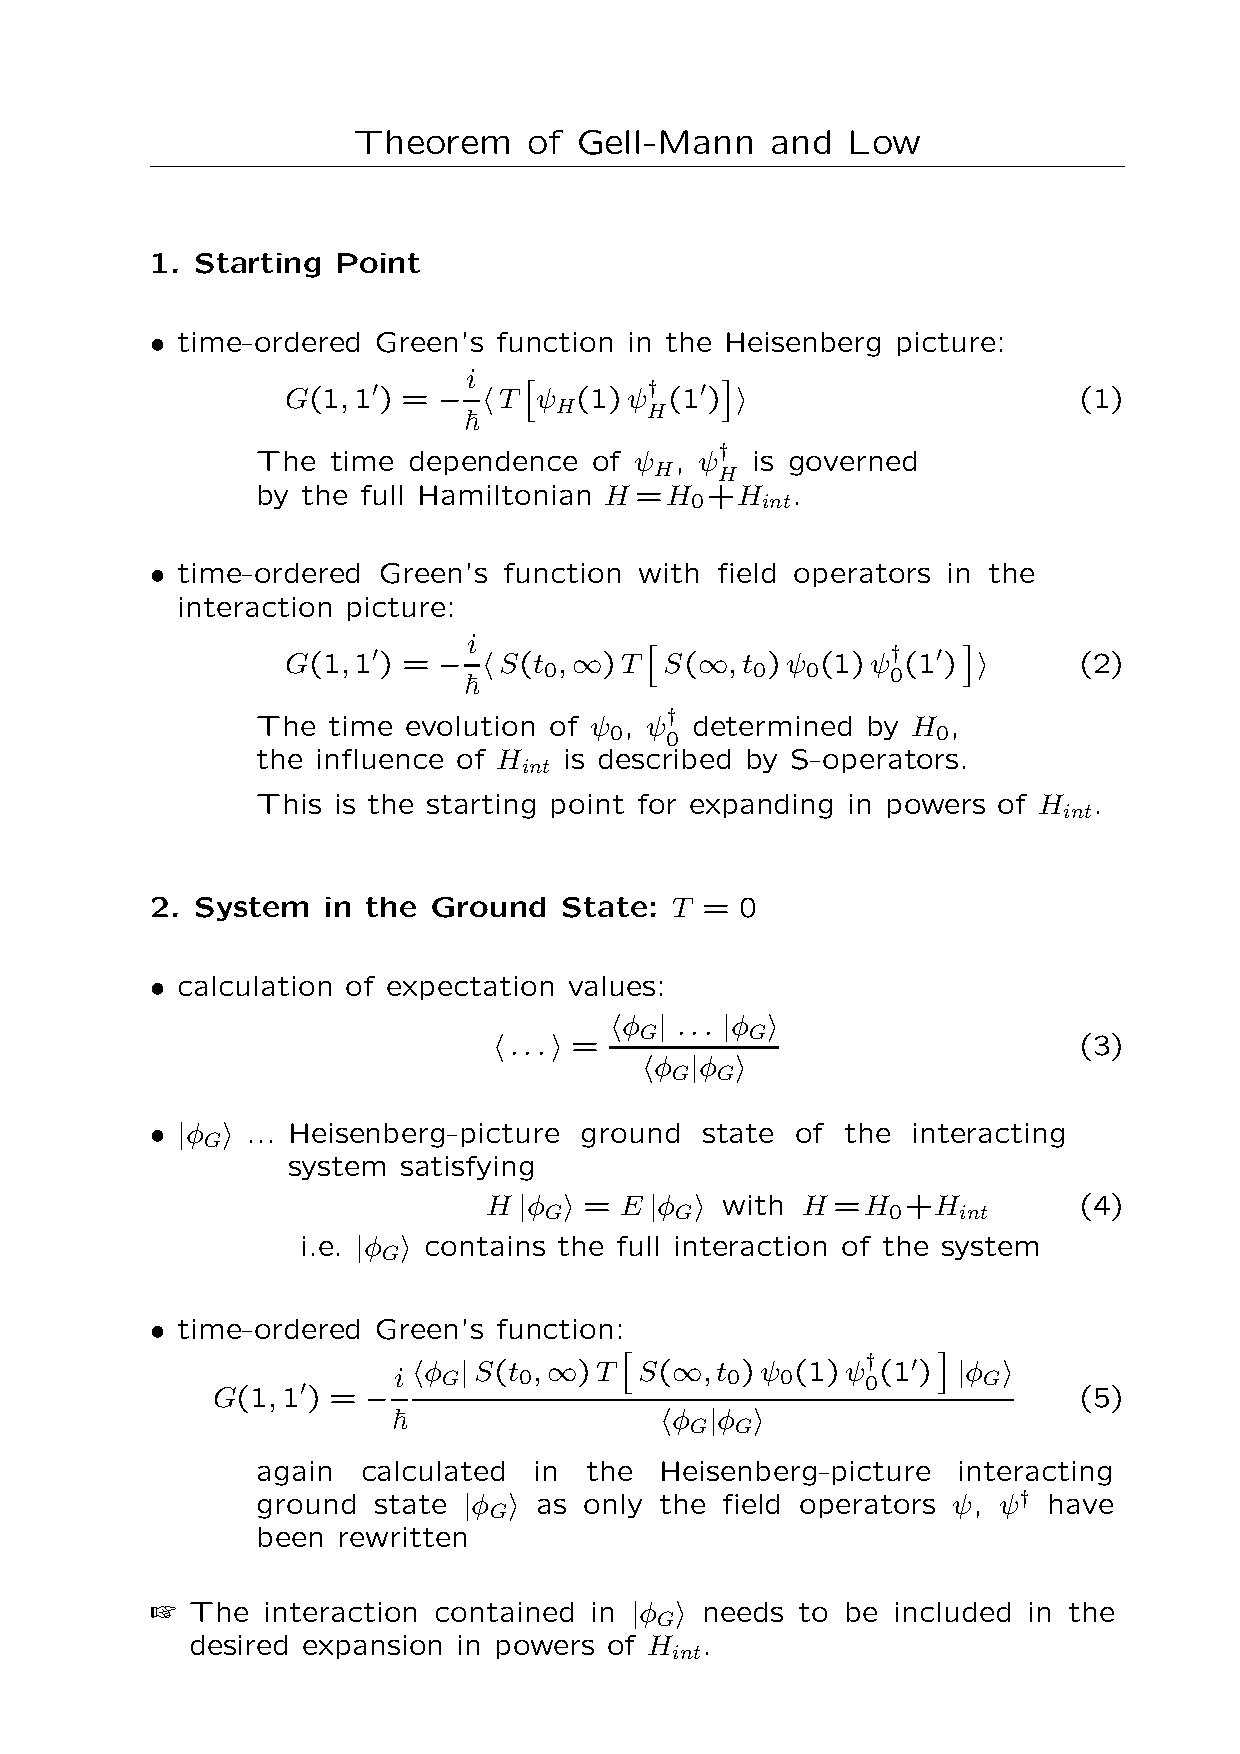
\includepdf[pages=1-3,pagecommand={},fitpaper=true]{PDF/Theorem_von_Gell-Mann_and_Low.pdf}
\clearpage
\subsubsection*{Anmerkungen/Notizen meinerseits}
\begin{itemize}
  \item Was wir mehr oder weniger gemacht haben ist die antizeitgeordneten Operatoren in zeitgeordnete Operatoren umzuwandeln,
        indem wir sie in den Nenner geschrieben haben.
\end{itemize}

\lend{Vorl. 27.04.2026}